%%%%%%%%%%%%%%%%%%%%%%%%%%%%%%%%%%%%%%%%%%%%%%%%%%%%%%%%%%%%%%%%%%%%%%%%%%%%%%%%%%%%%%%%%%%%%%%
%% Description:       Programmentwurf advanced software engineering
%% Author:      Manuel Berg, m.berg@enbw.com
%%  -*- coding: utf-8 -*-
%%%%%%%%%%%%%%%%%%%%%%%%%%%%%%%%%%%%%%%%%%%%%%%%%%%%%%%%%%%%%%%%%%%%%%%%%%%%%%%%%%%%%%%%%%%%%%%

\titlespacing*{\chapter}{0pt}{-30mm}{10pt}
\titleformat{\chapter}[display]
  {\normalfont\bfseries}{}{10pt}{\Huge\thechapter.\quad}
  
\chapter{SOLID (8P)}
\pagestyle{scrheadings}
\clearscrheadfoot
\pagenumbering{arabic}
\setcounter{page}{3}
\ofoot[\pagemark]{\pagemark}
%\ohead[\headmark]{\headmark}
\onehalfspacing

\section{Analyse SRP (3P)}
\emph{[Jeweils eine Klasse als positives und negatives Beispiel für SRP; jeweils UML der Klasse und
Beschreibung der Aufgabe bzw. der Aufgaben und möglicher Lösungsweg des Negativ-Beispiels (inkl.
UML)]}

\subsubsection{Positiv-Beispiel}
\begin{figure}[htbp]
\centering
\centerline{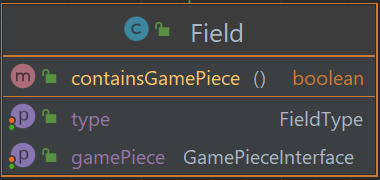
\includegraphics[scale=.6]{positivbeispiel_srp}}
\caption{Positiv-Beispiel SRP [Eigene Darstellung aus \emph{IntelliJ}]}
\label{fig:positivbeispiel_srp}
\end{figure}
\noindent Die Klasse \emph{Field} stellt als einzige Aufgabe ein Spielfeld dar. Dieses kann einem Typen zugeordnet sein, und optional eine Spielfigur enthalten. Durch einen Methodenaufruf wird zurückgegeben, ob sich eine Spielfigur auf dem entsprechenden Feld befindet. Das Single Responsibility Principle wird durch die hier dargestellte Klasse nicht verletzt.

\subsubsection{Negativ-Beispiel}
\begin{figure}[htbp]
\centering
\centerline{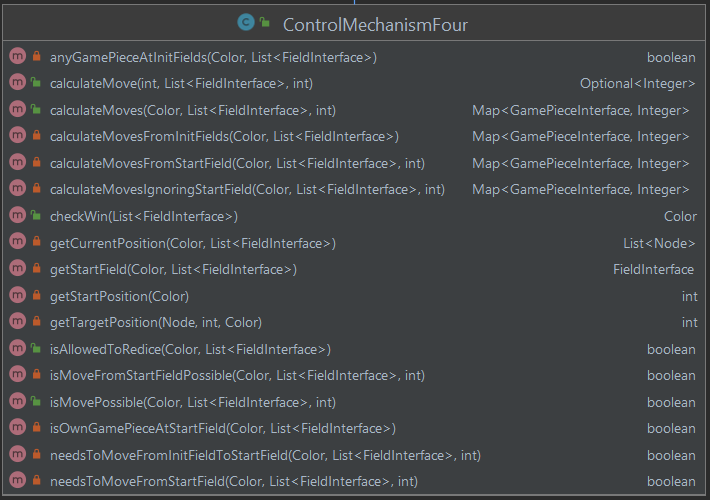
\includegraphics[scale=.6]{negativbeispiel_srp}}
\caption{Negativ-Beispiel SRP [Eigene Darstellung aus \emph{IntelliJ}]}
\label{fig:negativbeispiel_srp}
\end{figure}
\newpage
\noindent Die Klasse \emph{ControlMechanismFour} ist dafür verantwortlich, 
\begin{itemize}
\item mögliche Züge zu berechnen,
\item zu prüfen, ob ein Spieler bereits gewonnen hat,
\item zu prüfen, ob ein Spieler nochmals würfeln darf und
\item zu prüfen, ob ein Spieler überhaupt einen Zug durchführen kann.
\end{itemize}


\noindent Es wird deutlich, dass die Klasse für mehrere Tätigkeiten verantworlich ist und somit das Single Responsibility Principle verletzt wird. Um das Prinzip einhalten zu können, sollte der Umfang der Klasse auf die Erfüllung einer einzigen Aufgabe reduziert werden. Hierzu könnte \emph{ControlMechanismFour} in zwei neue Klassen aufgeteilt werden. Dabei wäre eine Klasse für die Berechnung der Züge verantworlich; die andere prüft das weitere mögliche Vorgehen eines Spielers. 

Außerdem enthält \emph{ControlMechanismFour} sieben private Methoden, welche in eine Hilfsklasse ausgelagert werden sollten. Diese privaten Methoden sind in \hyperref[fig:negativbeispiel_srp]{Abbildung 3.2} mit roten Schloss-Symbolen gekennzeichnet. Eine Auslagerung ist sinnvoll, weil die Methoden nicht nur in \emph{ControlMechanismFour} Verwendung finden, sondern auch in anderen Klassen (wie beispielsweise in der \emph{Graph}-Klasse) aufgerufen werden. Hierdurch wird redundanter Quellcode eingespart.

\newpage
\noindent

\section{Analyse OCP (3P)}
\emph{[Jeweils eine Klasse als positives und negatives Beispiel für OCP; jeweils UML der Klasse und
Analyse mit Begründung, warum das OCP erfüllt/nicht erfüllt wurde – falls erfüllt: warum hier
sinnvoll/welches Problem gab es? Falls nicht erfüllt: wie könnte man es lösen (inkl. UML)?]}
\subsubsection{Positiv-Beispiel}
\begin{figure}[htbp]
\centering
\centerline{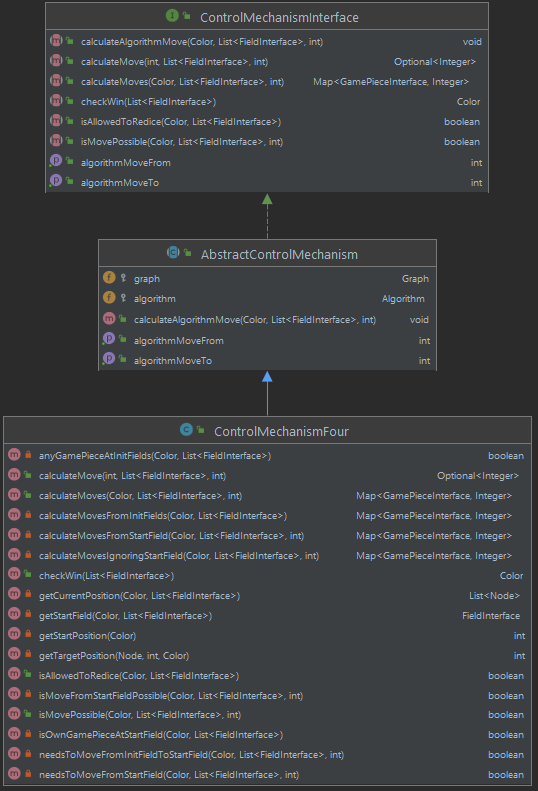
\includegraphics[scale=.5]{positivbeispiel_ocp}}
\caption{Positiv-Beispiel OCP [Eigene Darstellung aus \emph{IntelliJ}]}
\label{fig:positivbeispiel_ocp}
\end{figure}
\noindent Der \emph{ControlMechanism} ist offen für Erweiterungen bezüglich der Spieleranzahl. Dies wurde so entwickelt, da eine Abweichung von der Spielerzahl vier (z.B. Erhöhung auf sechs Spieler) eine optionale Anforderung des Projektes ist.
\newpage
\noindent Um beispielsweise einen \emph{ControlMechanism} für sechs Spieler umzusetzen, muss analog zur Klasse \emph{ControlMechanismFour} eine Klasse \emph{ControlMechanismSix} implementiert werden. Diese würde dann auch von \emph{AbstractControlMechanism} erben. 

Die Methoden werden immer über das \emph{ControlMechanismInterface} aufgerufen. Das bedeutet, ohne Änderungen an diesem kann das Verhalten wie oben dargestellt erweitert werden. Die OCP-Regel der verschlossenen Module gegenüber Modifikationen ist hierdurch erfüllt.

\subsubsection{Negativ-Beispiel}
\begin{figure}[htbp]
\centerline{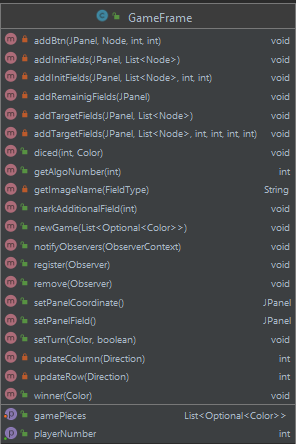
\includegraphics[scale=.6]{negativbeispiel_ocp}}
\caption{Negativ-Beispiel OCP [Eigene Darstellung aus \emph{IntelliJ}]}
\label{fig:negativbeispiel_ocp}
\end{figure}
\noindent ToDo: Negativ-Beispiel, weil wir hier nicht auf andere Spieleranzahlen erweitern können (Grafik)

\newpage
\section{Analyse LSP/ISP/DIP (2P)}
\emph{[Jeweils eine Klasse als positives und negatives Beispiel für entweder LSP oder ISP oder DIP); jeweils
UML der Klasse und Begründung, warum hier das Prinzip erfüllt/nicht erfüllt wird. Anm.: es darf nur ein Prinzip ausgewählt werden; es darf NICHT z.B. ein positives Beispiel für LSP und ein negatives Beispiel für ISP genommen werden]}

\subsubsection{Positiv-Beispiel DIP}
\begin{figure}[htbp]
\centering
\centerline{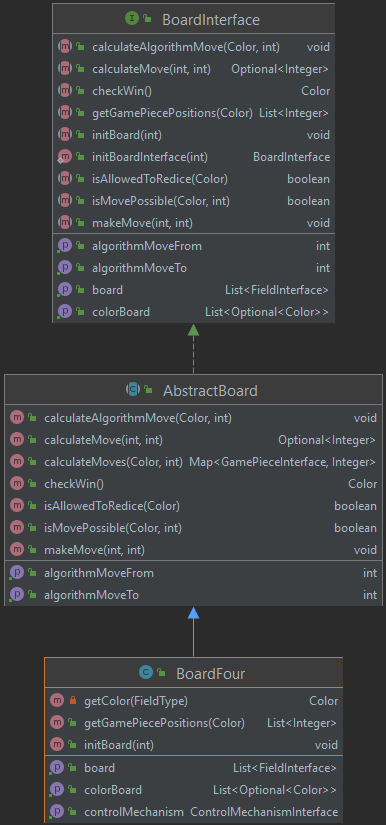
\includegraphics[scale=.45]{positivbeispiel_dip}}
\caption{Positiv-Beispiel DIP [Eigene Darstellung aus \emph{IntelliJ}]}
\label{fig:positivbeispiel_dip}
\end{figure}
\noindent Durch die Abstraktion des Spielbretts wird das Dependency Inversion Principle erfüllt, denn hier hängen die Details von Abstraktionen ab. In \hyperref[fig:positivbeispiel_dip]{Abbildung 3.5} ist zu erkennen, dass die Details -- also die konkreten Implementierungen -- in der Klasse \emph{BoardFour} zu finden sind.

\newpage 
\noindent Der Methodenaufruf beim Spielbrett ändert sich demnach nicht, wenn die konkrete Implementierung verändert wird. Beispielsweise könnte auch ein weiteres Spielbrett umgesetzt werden, ohne dass sich am restlichen Programm etwas ändert.

\subsubsection{Negativ-Beispiel DIP}
\begin{figure}[htbp]
\centering
\centerline{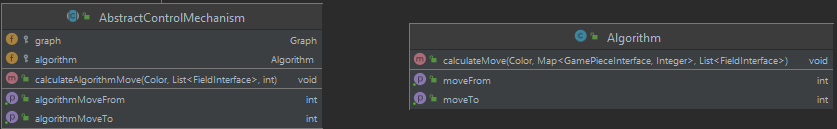
\includegraphics[scale=.6]{negativbeispiel_dip}}
\caption{Negativ-Beispiel DIP [Eigene Darstellung aus \emph{IntelliJ}]}
\label{fig:negativbeispiel_dip}
\end{figure}
\noindent Der \emph{ControlMechanism} steht in direkter Abhängigkeit der Klasse \emph{Algorithm}. Falls sich die Implementierung letzterer ändert, so muss auch \emph{AbstractControlMechanism} entsprechend angepasst werden. In dieser Zusammenstellung kann nur der vorhandene Algorithmus angewandt werden. Um dies zu umgehen und weitere Algorithmen verwenden zu können, wäre ein Interface sinnvoll.